\chapter{Living (and working) through austerity: everyday life for frontline workers and care-experienced young people}
\label{ch:5}

\section{Introduction}
\label{sec:5-intro}

In chapter \ref{ch:4}, I introduced The Charity and the three projects I worked with throughout my research - Small Steps, Building Bridges, and Seabird. Each of these projects claims to be grounded in the values of pursuing the best outcomes for young people and being young person-led, yet I began to notice slippages in the values of these projects. To answer my first research question, and understand the experiences and affects elicited by capitalist realism, in this chapter I explore the influence of austerity-intensified capitalist realism through a closer look at the experiences of frontline workers and young people within these projects.

Throughout the chapter, I recount stories from my fieldwork with Small Steps, Building Bridges, and Seabird, to understand the experiences of receiving support when perceived to be vulnerable, and the experiences of the workers who give that support. What happens to you if you are considered to be vulnerable? How are you treated? What does it mean to work with someone you perceive to be vulnerable, particularly in a time of rising pressures in your workplace? Through exploring these questions, I detail the affective and material impacts of austerity-intensified capitalist realism. I find that austerity-intensified capitalist realism has brought about changes to work, labour, funding, and temporal experiences. The changes made to the funding of charities generally - and support work with young people perceived to be vulnerable specifically - have resulted in there being more work to be done, with less funding, across the same or less time, with the same or less labour to do the work. I explore the ways this dynamic has affected The Charity, and how this is indicative of a wider shift within the third sector/social care landscape. 

I start the chapter with a vignette exploring the interconnected nature of these pressures. First, I recount the experiences and affects of those working with young people perceived to be vulnerable, before turning towards the experiences of those receiving support and who are perceived to be vulnerable themselves. I relate the experiences of frontline workers and care-experienced young people, and identify common themes of distrust, attempts to control, and feelings of disempowerment, anxiety, and isolation manifesting differently for each group. At the end of the chapter, I begin to question how austerity-intensified capitalist realism sustains these experiences and affects, exploring this through answering my second research question with the grounded theory of justification practices  in chapter \ref{ch:6}. 

\section{"I just have one or two thoughts on what we might want to do differently…"}
It is January 2019. Karen, Mandy and I arrive at our weekend’s accommodation – the cold, damp, yet somehow cosy Tregethan House. The weekend's residential hasn’t even started yet and we are already soaked through. The weather has been awful all week, but it's taken a turn for the worse today, preparing to make our jobs for the weekend much harder. We are soon joined by Michael, who pulls up to Tregethan in an expensive rental car, boot filled with snacks, games and DVDs. He is dry as a bone, and we try not to pay too much attention to the disconnect between us, the soaked delivery staff, and Michael, the dry senior manager. We gather together in the front room of Tregethan – which over the course of the residentials becomes known as "The War Room" – to set out the plan for the weekend.

Tregethan House is a large house owned by an outdoor activities charity,  who work with corporate teams and groups of young people (pictured in figure \ref{fig:tregethan}). The outdoor activities charity runs its team-building events for large companies in the main house, Trelawney House, whilst young peoples' residentials take place on the edge of their land, in Tregethan. The building is like every other space that I enter that is dedicated to running activities for young people: slightly under-maintained, but well-loved. The downstairs rooms are sparse, a stray sofa here and there, and a tiny kitchen filled to the brim with standard-issue 200ml glasses, too small to quench anyone's thirst. The bedrooms are filled with bunkbeds that feel slightly too small for anyone on the residential. More than once throughout Building Bridges' residentials, there are arguments about who gets to sleep in which room. 

\begin{figure}
    \centering
    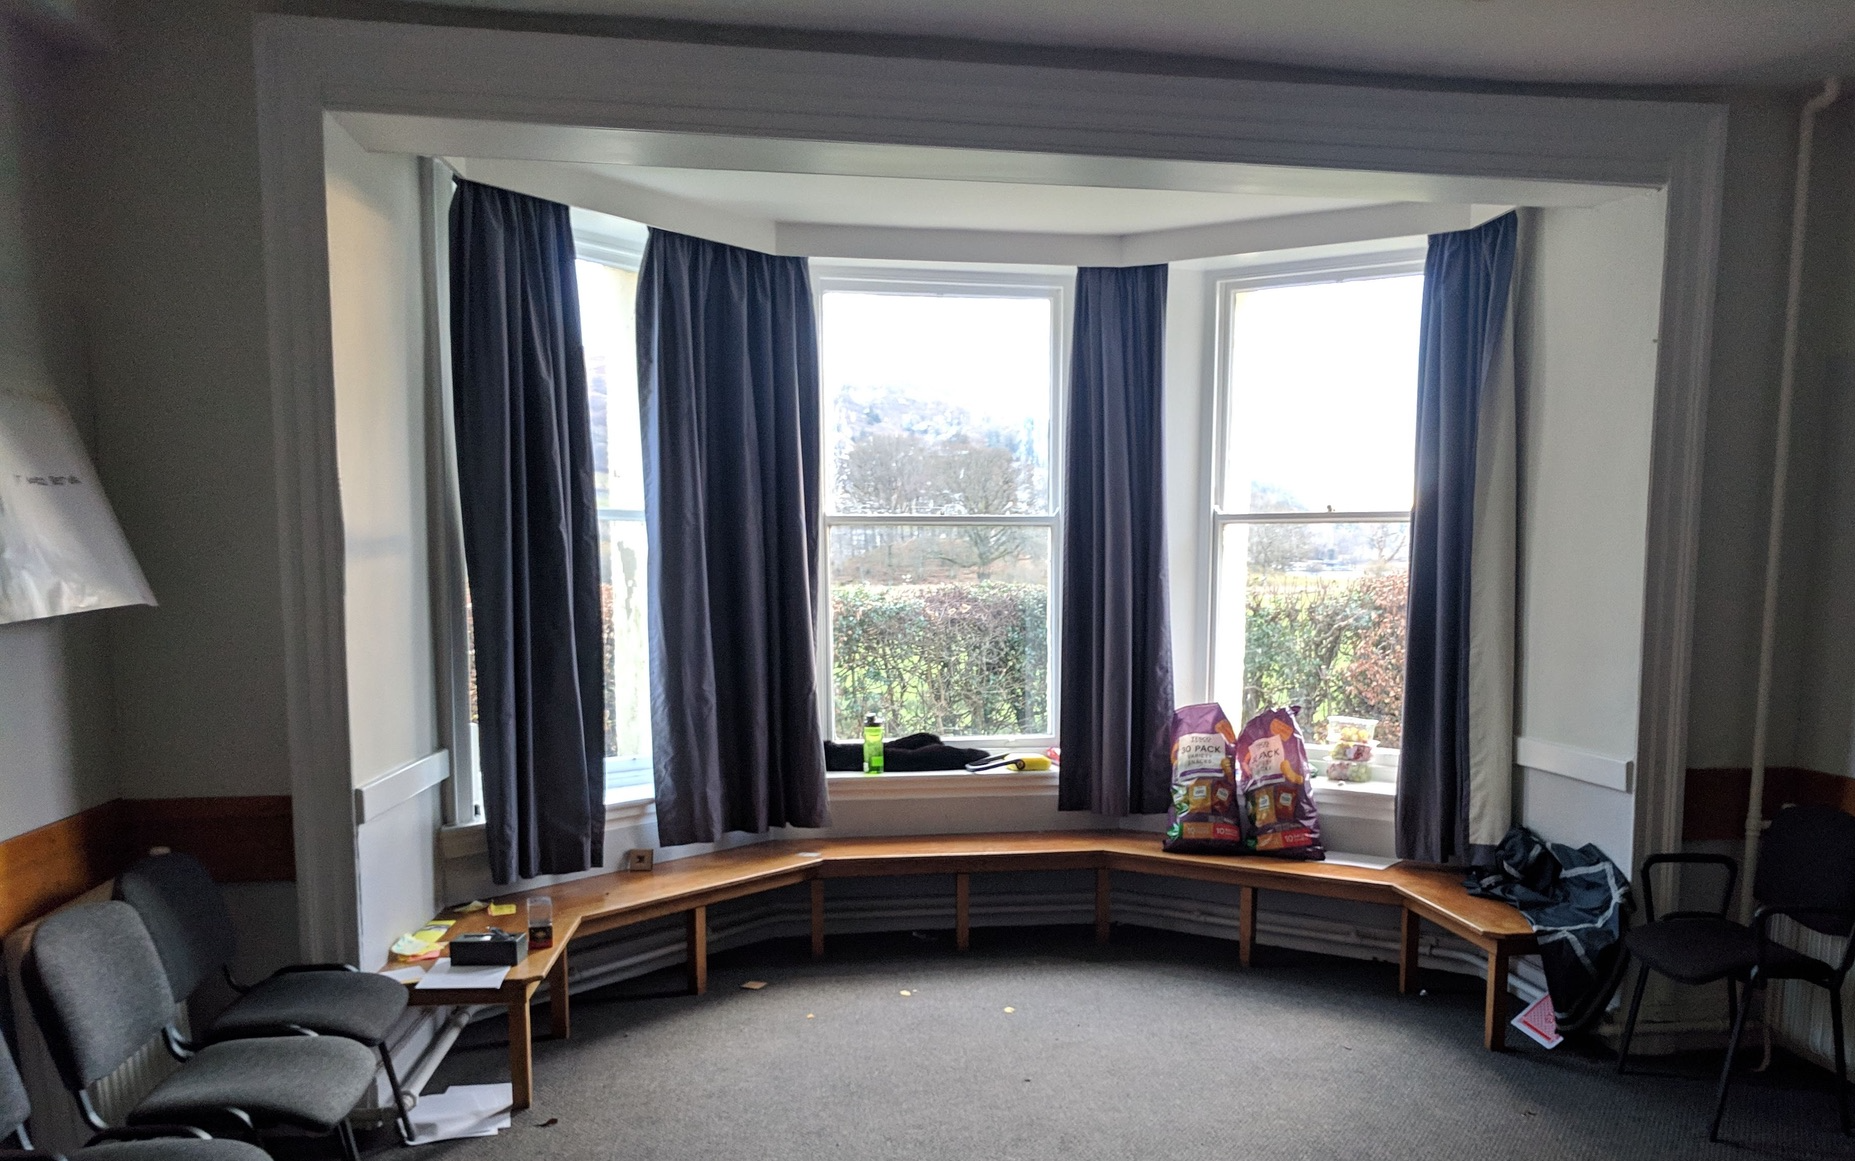
\includegraphics[width=1\linewidth]{Images/2/tregethan.png}
    \caption{The back room of Tregethan House, where most of the indoor activities took place.}
    \label{fig:tregethan}
\end{figure}

There's a familiar patter to our routines arriving at Tregethan. Karen, Mandy and I get there first and have a catch up - sometimes sharing a taxi from the nearest train station. Karen will recount a hilarious anecdote from her life, Mandy will good-naturedly make fun of me , and I am scrambling to finish writing a conference abstract at the last second. Then Michael arrives and we scurry into planning mode, despite the weekend already being planned. Karen explains the plan for the weekend in meticulous detail, with plenty of alternatives considered for everything. She's an incredibly skilled youth worker, despite occasionally doubting her ability, and she knows that you need options, otherwise you'll be derailed in the first ten minutes of the weekend and will spend the rest of the time trying to get back on track. Around halfway through Karen explaining the plan, Michael will cross his arms and start to look a little troubled. When he’s stressed, he has a habit of reaching towards his face and stroking it pensively while he decides the most opportune moment for him to speak. He strokes his face for a while. We get closer to the end of Karen’s plan, and then Michael stops looking as serious, and speaks:
\begin{quote}
Karen – this is a brilliant plan. You’ve thought of everything.
\end{quote}
A pause. 
\begin{quote}
I just have one or two thoughts on what we might want to do differently…
\end{quote}
He always says he wants to make some small changes. He'll reassure Karen that her plan is brilliant, he’s just concerned about a couple of things. Yet once he starts speaking, it’s never just a couple of things. Slowly, the whole weekend develops flaws, or unconsidered things. We can’t do that activity because of the weather. Those two young people can’t share a bedroom because they fell out last time. We’re going to want to keep an eye on those two young people because they spent half of the weekend smoking weed last time. Is this activity appropriate for everyone? What about the walk up the mountain, Mark isn’t going to do that, is he? 

These first changes tend to consist of critiquing the content of the activities. These sorts of perceived issues could perhaps have been ironed out if Michael had any time to actually manage Karen - he is finding it increasingly difficult to make sure he has time to comment on residential plans before he's on them, because of all the national travel and endless WebEx calls he finds himself on. Then, the the structural changes start to emerge:

\begin{quote}
I’m not sure we’re quite hitting enough of the transformational change side of things at the moment Karen. That’s not your fault, I don’t think I was clear enough. But we really need to capture their hearts and minds with this. Building Bridges is absolutely about those fireworks, those Trojan horses making local change. And if we’re not spending enough time on the missions I don’t just know if we’ll get that.
\end{quote}

Later in the weekend, when things inevitably start going wrong – because the well-planned, youth-and-social-work-centred activities have disappeared in favour of corporate priorities – Karen manages to find moments to feel bolder. In her version of the plan, we could account for some young people not wanting to take part in an activity, someone disappearing for a few hours (it happens more often than anyone would admit), or a sudden rebellion, a change of mood amongst all of the young people. There was space and alternatives accounted for in Karen's plan. We could let people get dry and have a hot chocolate after they got caught in a storm. When we follow Michael’s plan - with none of the weeks of consideration and balance, geared towards corporate priorities -  we end up constantly chasing our tails, trying to fit more activities into the weekend than we ever could have ever reasonably managed. The weekend becomes an anxious, confusing mess as we continually re-plan the activities every few hours – and oddly enough, end up delivering a residential that looks a lot more like Karen’s plan did in the first place. There’s always barely enough time for me to run an evaluation session at the end of the residential, which is the entire reason I’m here. Evaluation and reflection falls by the wayside in favour of corporate priorities. 

The young people arrive, and we will settle into an evening of getting to know each other again. On this particular residential, we manage to get to bed before 1am, a new achievement. The next morning at breakfast, Karen and I sit down to our watery-yet-somehow-overcooked scrambled eggs (a food that only residential accommodations and hotels are capable of making) and I ask her how she slept. She tells me:

\begin{quote}
I didn’t sleep too bad - y’know how it is on these beds! They’re always so hard. Though at one point – you’ll love this – I had a dream that I woke up  to Michael just hounding me, right in my face, saying ‘What’s the plan, Karen? What’s the plan?’ and – Mandy, you tell it, you were there -
\end{quote}
Mandy responded:
\begin{quote}
Karen just woke up saying ‘I don’t know where the plan is, I don’t know!’ It was hilarious.
\end{quote}
It was funny - I had an image in my mind of Michael’s concerned face popping out at Karen like a broken cuckoo clock. Yet I had the feeling we were laughing because of the truth of the moment. Karen was visibly exhausted as she recounted her dream. Constantly tweaking and changing the plan to bow to Michael’s whims \emph{was} tiring. I had experienced it myself, but Karen always bore the brunt of it. Karen and Michael got on well - Michael was her manager, but afforded her a lot of autonomy and support, and Karen always spoke about how much she appreciated that at that point in her career. They both respected each other and their respective professional expertise a lot. They spoke a good amount – maybe not as much as Karen would have liked, but it definitely was often enough to catch issues like the residential plan not being `transformational' enough. At each residential, the pattern repeated itself. Karen would painstakingly craft a plan, grounded in the needs of the young people we’re working with, and then Michael would come in at the last second with some concerns. This would continually play out: you think you know what you’re doing… and then you’re made to change the plan at the last second. You’re constantly busy, changing or tweaking something, and then you get to the point of running your event and you have to change it all again. 

I could tell that Michael really wanted to trust Karen’s plan – he was really hoping that he would just feel comfortable enough to say "yes, great plan Karen, let’s do it". Yet he could never quite let himself surrender to her plan, because to do so would require him to surrender control to Karen – to trust in her expertise and let her do what she had planned, informed by her years of experience by a participation worker and training as a social worker. The thought seemed to always be in the back of Michael’s mind: what if she gets it wrong? What if something bad happens? Ultimately, regardless of whose plan it was, Michael knew that the buck would stop with him - he was the team's Innovation Leader.  If something went wrong, didn’t go according to plan, or they couldn’t extract key outcomes or metrics from it, he would be the person held `accountable', or who would have to pay the price - whatever that might be. 

I witnessed this inability to surrender control all across The Charity. Workers struggling to open up to their managers, to tell them that they’re giving them too much work, that they don’t know what's expected of them. Managers struggling to believe in their workers. Young people refusing to trust their workers, thinking that they’re never going to listen to them. Workers refusing to listen to their young people, thinking that they’re just trying to get as much out of them as they can. Once this seed of distrust has been planted, it quickly grows into other experiences and practices, which can sow further seeds of distrust. Let’s take Michael as an example. He started his role in Building Bridges with an immense amount of faith and optimism, believing that he was going to make a difference for as many care-experienced young people as he could, and that he would be able to do so in a way that defied The Charity's complex bureaucracy if needs be. Yet he quickly became another cog in the machine, the pressures of his job kept catching up to him. He became unreasonably busy. It became incredibly difficult to get a meeting with him, because he’d be four different places across the country in a single week. At the same time, he was getting a lot of pressure from his bosses - The Charity’s Leadership Team - who wanted to see `results'. He was spending a lot of money on his programmes - and they weren’t seeing any improvements in people’s experiences to match that money. This ran directly counter to the values of the Central Services Innovation Fund, who funded this work. Its intentions were to use unrestricted finance to deeply invest, long-term, in some key areas of work without the threat of removal of funding, the need to track outcomes and outputs in conventional ways, in order to transform social care.

Michael’s good intentions began to give way to the constant pressure. At first, he told the Leadership Team that it would take a while to see improvements - that these were meant to be long-term projects, and they were interested in closely following what unfolded over time. Their pressure for `results' continued to increase. Instead of Michael reiterating the programme's values to them, he began to tell them that results were coming soon, or simply tried to avoid their questions. To take some of the pressure off of himself, he needed to start seeing some improvements that he could report back to his bosses. He started exerting that same pressure they put onto him. Instead of holding the line against these changes, he began to redirect the programme’s efforts to generating results - discussing different ways the programme could track outcomes, whether I could develop a digital to track mission progress, always making sure that photographs were taken so there was documentation of "all the great work we’re doing". As he exerted this pressure, then, the team began to feel it - worrying about whether the programme was achieving anything, wondering if they’d taken enough pictures, whether the evaluation data I was collecting was enough to get a sense of their impact.

In turn, Karen in particular took on ever more work, in an attempt to deliver on the outcomes they promised to deliver. In other projects within The Charity, I saw this play out again: either workers would make themselves busy, trying anything in an effort to demonstrate their impact; or, workers would try to resist the horizon of busy-work by \emph{looking} busy to attempt to avoid being burdened with more work. Those that do take on this work begin to take on an increasing amount of responsibilities that they are often not trained for. Karen had to co-ordinate the programme’s national network event, and act as a supervisor to the frontline workers on Building Bridges, despite not wanting to do so. More labour is being done than ever before, but even more labour is required than before. This busy-ness gives way to stress and anxiety as people hit `capacity'; as time goes on, stress and anxiety metamorphose into burnout. Sometimes, people want to leave, but they feel like they owe too much to the organisation and the people it supports. Some try to ease up the workload by sharing it with others, but it becomes so difficult to collaborate because there is so much work and everyone is working at capacity all the time on things they know nothing about, so they can’t collaborate or share even if they wanted to. They feel lost, isolated, and alienated.

Underlying these experiences is a lack of trust. You want to tell your manager you’re too busy but you can’t, because you don’t believe anything would change if you do. You want to tell your funders the situation has changed and you can’t deliver what you proposed but you can’t, because you’re terrified they’ll retrospectively remove the funding and the organisation will be broke. You want to tell your teammate that you’re burning out and feel like you’re always drowning under the weight of the work, but you’re terrified they’ll think less of you. It turn, it begins to affect the service provision and the young people who should be supported by it - they too feel lonely, isolated, disoriented and anxious because their workers are constantly too busy to listen to them properly and make the changes they need. They wonder why no-one is supporting them, or why it feels like they can never get what they need. They might even begin to feel as if it’s their fault that things are like this, or that they deserve it. This is what the contemporary care system looks like: cycles of managers taking on too much work to try to keep their organisation afloat, passing the pressures onto workers, who pass the pressures onto young people, and all the while everyone becomes affected by it: confused, anxious, stressed, isolated, exhausted. In the next section, I explore the experiences of those who work with people perceived to be vulnerable in greater detail, and identify how their experiences lead to these negative affects. In the following section, I do the same for young people perceived to be vulnerable and identify the commonalities between these experiences. 

\section{Being a `worker': the experiences of care work under austerity-intensified capitalist realism}
Across The Charity's different projects, managers and workers alike are affected by austerity-intensified capitalist realism. The lack of trust described in the preceding vignette is facilitated by the high-stakes environment brought about by the ‘value for money’ described in chapter \ref{ch:2} and its renewed focus on programme evaluation. If an organisation wishes to demonstrate value for money, then they must identify a change in either the time they deliver a project for, the cost of a project, or the scale of its intervention. These can be thought of as changes to work, labour, time, and money\footnote{Here, I am referring to \textit{work} as a project's scale and required labour, \textit{labour} as the amount of available workers to do this work, \textit{time} as the duration of a project, and \textit{money} as the project's cost or budget}. To briefly demonstrate the forms these changes might take, let us briefly consider two organisations. Organisation A can deliver a service for £100,000 to 65 young people across a one-year period. Organisation B can deliver a service for £70,000 to 65 young people over a one-year period. Organisation B would be considered to be creating greater value for money. The options available to organisations, then, are to:
\begin{itemize}
\item Deliver a smaller service for the same cost as another organisation,
\item Deliver a larger service for the same or lower cost as another organisation,
\item Deliver the same service for a lower cost, 
\item Deliver the same service for the same money over a longer time, or
\item Create more evidence about a service's impact (which could be effective regardless of work, labour, time, or money).
\end{itemize}

In this chapter, I am most concerned with the impacts of this change, rather than these in specific. In the next chapter, I will explore some of the content of this change in greater detail. Throughout my research, then, these changes have led to three consistent experiences within my research with managers and workers within The Charity: 
\begin{itemize}
\item There is not enough (or the wrong kind of) labour to do the amount of work there is,
\item There is not enough time to do the amount of work there is, and
\item There is not enough money to source a sufficient amount of labour. 
\end{itemize}
Although these are all interrelated, each of these experiences of work, labour, time and money emphasises a different aspect of this change. For example, there not being enough labour to do the amount of work there is highlights how managers adopt control techniques to ensure that work gets done, resulting in workers having to do things they aren’t trained for, there being low organisational capacity and workers feeling stressed, anxious and burning out. There not being enough time to do the amount of work there is highlights how workers’ experiences of time shift, with a tendency towards experiences of acceleration or contraction, where time speeds up and not enough can be done in that time. Finally, there not being enough money to source a sufficient amount of labour highlights how organisations can focus on commercialisation or constantly attempting to secure more grant funding, in order to secure the future of their organisation - yet when new funding comes in and there are more workers, there is no decrease in the overall labour that must be done. Although each of these different emphases add a unique dimension to our understanding of the changes brought about by austerity-intensified capitalist realism, I will explore only the first of these experiences in this section in the interests of length\footnote{I detailed the impact of changes to worker's temporal experiences in a conference presentation at the British Sociological Association's Annual Conference in 2021}. This does come at the cost of exploring how workers' experiences of time have shifted, and how workers have come to view their roles in financial terms, but the focus on the lack of available labour is sufficient to understand the dynamics within The Charity. 
 
Workloads in The Charity are incredibly high. For people that work directly with young people, this might involve high caseloads of 25 or more\footnote{Personal advisers (who this refers to) are expected to physically visit each person in their `caseload' at least once per month, along with providing support and filling in casenotes/paperwork for each person. }, or running multiple residential programmes sequentially; for people that might hold a more ‘strategic’ role where they have less contact with young people, this might involve taking on a steady stream of new projects, attending a large number of events, or filling every moment of a work day. It’s difficult to pin down exactly  what ‘too much work’ looks like, but it can more easily noticed through the traces it leaves: people not taking lunch breaks, scheduling back to back events in their calendar, trying to optimise their days, and feeling stressed, anxious, or disempowered as a result. In this section, I explore workers' experiences of `too much' work, and what results from this. This includes doing work that people aren’t trained for, the emotional labour and fallout that results from this high pressure environment, and the control techniques employed by managers to attempt to keep labour levels high despite all of these issues. I did also work with managers throughout this, but their viewpoints primarily feature in their position as workers, not managers. Managers are discretely discussed to talk about how they use control practices to manage the work of other workers.

\subsection{Doing work that you’re not trained for}
Because managers are constantly changing aspects of how projects within The Charity function, workers have to navigate a state of constant change. Managers may be applying for funding for new work, trying to enhance their project’s reputation, or build links with new organisations. Across each project in turn, I witnessed workers begin to feel that their project was taking on work that they had little to no capacity to deliver, or no pre-existing skillset that would aid with delivery. The disconnect between managers and workers mean that new work emerges with little consideration of the workforce's ability to do it. This might lead to people doing work that they are not trained for, but may also lead to a complex allocation of resources, where some worker's roles are funded by multiple different projects, and workers having to do a bit of everything. Whilst this is not intriniscally a problem, and could work well if well-supported, in the case of the workers I spoke to, it instead led to confusion and a lack of clarity. In the most severe cases,  some people felt a complete lack of identity to their role - ensuring that they found it incredibly difficult to focus on their role's specific remit, and led to them worrying about all aspects of the organisation.

Those responsible for bringing funding into their project will often make proposals with little consideration of the organisation's current ability to deliver the project. They will then either hire new workers or reallocate workers from project to project in order to make sure that it can fulfil its proposal if it is successful in its bid. Colin was a trained social worker, and was employed in Small Steps as a Regional Project Officer, primarily intended to deliver training courses to young people about novel psychoactive substances and healthy relationships, but much of his job consisted of writing blogs about what he had done rather than actually using his social work training directly with young people. Tina from Seabird was a youth worker with significant experience of direct work with young people, but when the organisation won the contract for their county’s participation work with care-experienced young people, she was forced to become participation lead. Tina had to work out how to run the Children in Care council with no prior experience, and although she ended up being good at her job, she had no idea what she was doing to begin with. Similarly, Karen from Building Bridges was a trained social worker and experienced youth group facilitator, but ended up taking on a variety of other roles within the project, such as researcher, programme manager, travel co-ordinator, and professional supervisor, with little support in each of those roles. Ed, a just-graduated marketing student working for Small Steps, acted as social media manager, designer, website editor, personal assistant, and receptionist. Workers at The Charity are moved from project to project with little consideration for their preferences or skills. One month, a worker may have been trying to support young people to get into employment, but the next month they would be  trying to help them with their mental health. Practice is forced to follow where the money is.

Workers are moved between projects with little consideration for their existing skillsets, filling whatever gaps in delivery capacity might exist. People's relative skillsets are not largely considered: the work simply needs doing. The workforce remains composed of the same people, hopping around from task to task. Sometimes this just involves a defined role taking on additional responsibilities (as in the case of Ed and Colin), but this also takes the form of complex resource allocation, where someone has two or three defined roles, flexibly using small amounts from each fund that a project has access to in order to fund a day of someone’s time on each initiative. On paper, Nellie's role in Seabird was funded from a single initiative’s funding, but in reality, she worked on two other initiatives too, and the workers responsible for those initiatives also worked on Nellie’s initiative. This resulted in many of the staff members at Seabird doing a "bit of everything" in Nellie’s words. 

To some extent, this might be considered an innovative response to the restrictions of many funding schemes. Yet the impacts of this practice lead to greater harm for workers, creating a lack of clarity around the responsibilities contained within their individual roles. At best, workers might feel confused at this ambiguity, but the extra cognitive load of being ambiguously responsible for three simultaneous projects can create much worse affects, along with extra work. Tina felt constantly stressed, as she struggled to meet the demands of multiple projects at once, whilst feeling she was unskilled at all three. Both Ed and Colin struggled to explain their job roles when I asked them, and didn't feel as if they knew what was expected of them except for what Shelly asked for. This lack of identity even made their day-to-day work more difficult on several occasions, as being unable to easily explain what their organisation did to external organisations, and prevented them from making crucial connections. Early into my relationship with Colin, I asked him to explain what the organisation was about and what they did, in order to get a better sense of  Small Steps from his perspective. He struggled to answer. I would ask him the same question intermittently as we worked together, to see if things had got any clearer. Once, he attempted an answer, but he concluded with "but I’m not even sure if that’s right!" Later in my research, Colin left Small Steps to work at a local authority as a personal adviser - a role which at least slightly used his social work training. Once he started his new job at the local authority, I met up with him and asked him to reflect on his time at Small Steps. He still didn't know how to explain what he did. He felt quite strongly that this had been part of the problem with the organisation - that he didn't even know how to explain what \emph{he} did, so how could he explain what the organisation did? 

%vol labour
% have found myself enfolded into these change processes time and time again, even when I have specifically avoided them. Much of the research that I will detail in the following chapters represents a partial enfolding of these processes and my work: they adapt to the priorities of the partner organisation, and then sometimes they adapt and adapt again. As Colin once explained to me, "they'll get every pound of flesh if you let them". Sometimes, these have been small pieces of work - a logo here, a survey there. Other times, they have been significantly larger - like the time I was asked to redesign Changemakers entire mode of service delivery, or to make a theory of change that explained their work and the impact that it hoped to make. These kinds of work go above and beyond what I had expected to do with these organisations, even taking into account my embedded positions with them.

This was concordant with what I had witnessed just before he left the organisation. Towards the end of my research with Small Steps, I interviewed Ed and Colin about how the organisation was operating at the time, as I had begun to notice a shift in their availability for working on our shared project together. Colin succinctly diagnosed what he felt was Small Steps’ problem:
\begin{quote}
At the moment, we try to do too much. We need to clarify what we want to achieve. Get a vision, some aims, a goal. We need that. It's also the size of us though... you know, we're tiny. And then if you have issues, you don't feel comfortable explaining them to Shelly. It's just you two. I feel like I can't be honest with her... hell, it's even hard to disagree with her.
\end{quote}
I interviewed Ed the next day. He echoed Colin’s sentiments, without having spoken to him:
\begin{quote}
Really, we're doing too much. We're doing more now than we ever were but with less capacity. Training? That was never really what we were about! We need to understand what we want to do. I don't know if we do the best right now... I don't know how to put into words what I even do. I'd never want to see the organisation go away. I believe in Small Steps. But we need to keep our core values. We're doing too much right now. Shelly thinks she can get everything done - she thinks she knows what she wants. But there's so much pressure... she just agrees to everything - but then we're the ones who have to do it.
\end{quote}
Both Randall and Colin felt like Small Steps was doing too much, and that the organisation needed to take a step back and clarify its purpose. They felt that Shelly was taking on too much work without a focus, placing ever-more pressure on Randall and Colin. Randall and Colin were struggling to get everything that Shelly wanted done, but they didn't feel as if they could tell her this. Their experience is indicative of how a worker might behave if a manager like Shelly assigns someone too much work, or work that they feel they are not trained for. One might silently accept the current state of affairs, because it feels to difficult to disagree with the manager, or because they don't feel comfortable explaining to them just how difficult they might be finding it to have no fixed set of responsibilities.  

Randall and Colin's case highlights how an organisation taking on `too much work' can lead to workers doing things that they have few skills in and little training for. As a result, managers directly worsen their employees' working conditions and the way that they feel both inside and outside of work. Worker voice begins to suffer, and this worker disempowerment begins to normalise this state of affairs, perhaps causing managers to think their workload expectations are reasonable, because they're not being told otherwise. Then, when workers begin to struggle, they don't tell their managers for fear of repercussions. In some cases, workers might lie to their managers to reassure them; in others, they might lie by omission, using the fact they're constantly busy to avoid giving any updates. Here, workers begin to outwardly perform how busy they are in order to either avoid negative repercussions or to avoid being given more work. 

This culture of appearing to be busy was most prevalent inside of The Charity’s head office. Mandy (a member of the Building Bridges team who was based in The Charity's head office) once remarked to me that the organisation was "full of people being busy, just to be seen to be busy". For the head office, this took the form of standing meetings that were never taken out of people's calendars that people were required to attend. In Mandy's words, these meetings were "a fucking waste of time" in which nothing ever got done - but people kept the meetings there, their purpose unexamined as they added to the performance of being busy. People would meet and talk on the same agenda items without anyone in the meeting gaining any greater understanding as a result. The high workload and low organisational capacity brought about by the value for money funding agenda thus results in a culture of both being busy (by doing work that people are untrained for) and appearing to be busy, which leads to confusion and a lack of clarity about individual responsibilities. This confusion can worsen, leading to negative affects such as anxiety, overwhelm, and even burnout. 

\subsection{The emotional labour of doing `too much work'}
Too much work being brought into the organisation leads to a culture in which workers' emotions are deprioritised, which takes a huge toll in a caring profession. Many of the workers I researched with reported extremely high levels of stress, anxiety, confusion and overwhelm. Care and support work is a field that naturally necessitates a high degree of emotional labour, "the management of feeling to create a publicly observable facial and bodily display" \citep[p. 7]{hochschild_managed_2012} in the specific context of paid labour. Professions which require a large degree of emotional labour risk the worker becoming "estranged or alienated" from their own body, since the the need to show only positive emotions commodifies the affective experience. Although initially Hochshild suggested that the work undertaken by social workers or other ‘caring’ professions would not strictly be classed as emotional labour because it doesn’t feature an "emotion supervisor" (through which the employer can enforce the management of emotions), recent work by \citet{leeson_emotional_2010} and \citet{winter_emotional_2019} suggests that emotional labour does occur in these professions, particularly in the context of a high degree of bureaucratisation. As explored in chapter \ref{ch:2}, austerity-intensified capitalist realism absolutely brings bureaucracy to the labour enacted in caring professions. As such, the management of emotions inside of The Charity can be understood as emotional labour, as workers are forced to police their external performance of emotions in order to deliver good care work.

In the context of austerity-intensified capitalist realism, then, this emotional labour is doubled: not only is there the emotional labour of having to appear calm and collected when working with people whose life circumstances may be incredibly difficult, but there is also the emotional labour of having to appear happy, calm and stable in a work environment which is creating the opposite of those feelings. Many of the workers I researched with felt constantly stressed or anxious, trying to meet the high workload assigned to them and feeling like it was their own fault or poor self-management of their time that was preventing them from doing so. When Colin eventually left Small Steps, he explained to me that a big reason he was leaving was that he wanted a job where he didn't feel confused or anxious about knowing what he was doing. Similarly, the story I recount in the opening vignette (of Karen dreaming about Michael shouting at her about the plan) came from a place of high stress and anxiety. Karen was in a state of high stress throughout the time I worked with her during Building Bridges, in large part because Michael often changed her plans at the last second, so she struggled to feel confident and secure in knowing what she was delivering.

%talk about humour as coping mechanism?
Tina from Seabird was perhaps the most significant example I encountered of this. When I was working with her, she was often unable to concentrate because she was always going over "the million things [she] had to do" in her head. It was a delicate balance that was easily disturbed. One morning, I came in to the office and found her flustered, intermittently going between her computer, a funding application, several phone calls, and other people's offices, trying to \emph{literally} do three things at once. I asked her if she was doing okay, and she merely responded "I've gone panic mode", and left the room. I spoke about that day to her a few weeks later and she explained to me: 
\begin{quote} 
That morning, I had so much going on, I just couldn't deal with any of it. You know, I got in that morning, I had a cup of coffee and just burst into tears. But hey, some days are just like that.
\end{quote}
It is easy to hear how Tina normalises the experience by suggesting that "some days are just like that". Clearly, whilst not an everyday experience, this was not the first time this had happened. The emotional labour of managing these affects is significant; the times that a worker like Tina actually lets these emotions be seen is when they fail to manage to perform the emotional labour any longer. Every panicked outburst or inability to focus is indicative of a more frequent experience of \emph{succeeding} in the performance of emotional labour - not letting one's colleagues or managers see how they are feeling, how difficult they are finding the workload. Their work environment is pervaded by a lack of trust, and as such workers become worried that others might see that they’re not able to do their work and that managers may get involved. In this way, the "emotion supervisor" of the initial theory of emotional labour becomes imagined or self-governed, forcing people to manage their emotions about the level of work and preventing any effective solidarity forming about the high level of work, for fear that you may be singled out. Again, in a caring profession this is compounded, as there are times when the need to appear as if there is nothing wrong is more important - centrally, when working directly with young people. Although some people may be fine with a worker sharing their authentic emotional state with them, it is incredibly important that the worker does not do so in such a way that would make the young person feel responsible for the worker's emotions. As such, these critical periods of emotional labour (in which the mask \emph{cannot} fail, or there will be negative consequences) increase the pressure a worker might feel. The changes brought about by austerity-intensified capitalist realism normalise this heightened affective state, where workers are used to being stressed, anxious, distrustful, confused and feeling disempowered.

It is no surprise, then, that the pressures of working in this environment makes many workers want to leave their jobs. This desire to leave, however, is often arrested by a sense of responsibility to the organisation or the young people that workers are supporting. When I spoke to Randall about the current state of Small Steps towards the end of our work together, he explained that he "really, really want[ed] another job", but was worried about what would happen to Small Steps if he (or Colin) left. Randall was aware that by doing a bit of everything, all of the workers had become essential to the functioning of the organisation, even if Shelly didn't realise this. On more than one occasion, Karen had wanted to leave her role in Building Bridges, but as the person responsible for co-ordinating the programme, she knew that she effectively was the project: if she left, the project would stop happening, and all of the important relationships she had built with young people and workers would fall away. Similarly, a year or so into my work with Seabird, a large number of people left either directly or indirectly related to the environment being created by managers. Randall left Small Steps eventually, but he felt deeply conflicted about it until the very end. His new role was with another charity in the building, and when he left Shelly joked that he would be down every other day to help them with tech support. Randall nervously laughed, and then just said "I don’t think I’ll be doing that". Under austerity-intensified capitalist realism, then, care workers not only have to do a significant amount of emotional labour (to their colleagues, managers, and their service users), but are often prevented from relieving much of the pressure they may be feeling due to the need to appear busy (as explored in the previous subsection) and the sense of loyalty that small teams often inculcate. Care workers are made to actively reperpetuate their own working conditions by not speaking about the issues they are experiencing, and feeling conflicted about the prospect of leaving. Ultimately, this is due to the environment that is created by managers.

\subsection{The control techniques used by managers}
Managers within The Charity tend to have the final say about how things get done. In some projects, like Building Bridges, there might be a manager above a manager that determines more about the work, but in others, managers have final say. Of course, managers are merely trying to find a way to effectively operate within a compromised system which has had its budgets cut and expectations raised. Workers doing things that they aren't trained for and experiencing an intensified emotional labour are ultimately the result of techniques employed by managers to attempt to continue delivering vital services, to ensure care work gets done whilst operating under an immense amount of pressure. Being a manager within The Charity is a curious position - you are still a worker, and therefore subject to all of the pressures and difficulties described in the preceding sections - but you are also responsible for the success of your project. If it doesn’t meet its outcomes, you’re the one to blame. If it doesn't produce sufficient outputs, you're the one to blame. In chapter \ref{ch:4}, I described how Small Steps would often compromise its co-production agenda by applying for funding and committing to a project without any input from young people, then consulting with young people afterwards and calling it co-production. I also described Michael’s strategy of letting Karen and I present our plan, uninterrupted, before laying out how he intended things to go - reminiscent of the "few concerns" he expressed in the opening vignette. These are both examples of the control techniques employed by managers. The techniques most used in my time with The Charity include using complex resource management techniques, constantly looking for ways to collect data from young people, and appearing to listen to workers yet disregarding them in practice. These are techniques of control because at their essence, they involve forcing or coercing someone to do something that they might otherwise not want to. 

Projects within The Charity use complex resource management techniques in order to get the most out of the funding available to them. I have already described how these techniques can result in workers’ jobs being funded from multiple streams, and how this can raise the amount of work a person has to do and lead to confusion in what someone’s specific role is. On top of this, though, there is a tendency to use these techniques to attempt to make work appear  linear, unchangeable, and "under control". Managers attempt to plan out when everything is going to happen, making it appear as if a project is going well and is running on-time, regardless of what is happening in reality. For Shelly, this took the form of a spreadsheet on her computer she referred to as "the Uber Plan". Though I was never allowed to see the Uber Plan directly, from what Colin told me and what I could infer from context, it acted as a complete record of everything Small Steps were doing. Grant proposal deadlines, outcomes reporting deadlines, new schemes of work, the daily ongoing tasks of Colin, Randall and Ronnie - everything went onto the Uber Plan. 

It isn’t out of the ordinary for there to be some kind of master plan or project management tool in place in an organisation. What was remarkable about the Uber Plan was the way that it became the central touchpoint for all work done in the organisation. Whenever anything happened, Shelly would go straight back to the Uber Plan. If you made a vague reference to "maybe being able to do something" - Shelly would commit you to it by putting it into the Uber Plan. It seemed at times that moderating and managing the Uber Plan was Shelly’s main function in the organisation. Her use of the plan seemed to function as an attempt to tie \textit{potential} events to \textit{specific} times, and in doing so create commitments from people, or at a minimum have a reason to check back in with someone. Whilst not as excessive, I also witnessed this in Building Bridges and Seabird, in the form of there being a greater focus on establishing timelines for work than doing the work itself. These are techniques of resource or project management being deliberately misused in order to try to create greater value for The Charity. They also contribute to a change in workers' temporal experiences, as timelines become compressed or accelerated. When timelines \emph{did} change, as they inevitably have to, the Uber Plan merely shifted retrospectively - as if to appear that the plan had always been for the project to proceed like this. This is an incredibly clear example of the "dreamwork" detailed in chapter \ref{ch:2} - there is a projection of a linear, accelerated future, and then when the projection fails because reality reasserts itself, a new narrative is presented about the past and present that suggests it had always been this way. There is no reflection on why the timescales needed to change, and often there was no record of the change. In part, this was due to an anxiety Shelly had about the project's reputation - she felt the need to project the image of a smooth, well-functioning organisation in the hopes of attracting funders. Any messiness - like changing timescales - might damage the project's ability to deliver "value for money". 

Fundamentally, the use of control techniques is an attempt to remove uncertainty or chaos from practices that are intrinsically uncertain or chaotic. As I will explore in the next chapter, the form this takes most often is in the creation of outcomes and outputs as the smallest unit of measurement of how a project is providing "value for money" and thus how they are meeting their funding requirements. This renders the actual work taking place secondary to the work of producing outcomes and outputs; the project could continue with minimal frontline practice occurring, in theory, as long as there were impressive traces produced of this practice in the form of outcomes and outputs. A variety of control techniques therefore focus on the introduction of methods of data collection (or extraction) about young people’s lives, experiences, or `progress'. Managers often want to know how a project is going, or how a young person is doing, but this can lead to a focus on data collection at inappropriate times or ways that disregard young people’s agency. My initial involvement with Building Bridges, for example, had been to explore the development of a tool that could help young people to track their progress over time as they worked on their missions. Michael was initially eager for a tool that helped young people to meaningfully reflect on the progress they were making on their missions \emph{as well} as gathering data for the evaluation of the programme. Yet as the project progressed and the pressure from Michael’s managers grew, he became increasingly interested in the design of a technology that would act as a "barometer". He didn’t even really seem to know what he meant by it - he just wanted a clear and visual set of metrics that he could show to his managers to say "this is how well they are doing". Similarly, when we were exploring the design of a digital peer support system in my engagement with Small Steps, Shelly repeatedly insisted that any such system should allow the organisation to use discussions had on a digital peer support system as data to include in funding proposals as evidence of engagement with young people - as mentioned in the previous chapter, she felt this was "too good an opportunity to miss". Yet the want to use this data for this purpose could delegitimise the tool's original intention - simply to create a space to support high-quality peer support. If a young person knew that everything they spoke about on a peer support platform might be used in a funding bid that they have no input into, they might be much less likely to engage with it. Here, there is a clear slippage between the project's stated values of co-production in service of the imagined future of the project's success. Shelly was willing to reduce the potential efficacy of the peer support service in order to \emph{potentially} help the organisation in funding bids - again acting as an attempt to remove uncertainty from places that are inherently uncertain.

A final control technique I witnessed within The Charity was the tendency to appear to listen to workers about their concerns or desires for the future, but ultimately disregarding them. Michael repeatedly did this (in the opening vignette of this chapter, or the lack of redesign of Building Bridges mentioned in the previous chapter, for example), and Shelly and Tessa did too. Shelly expressed this most clearly by saying one thing and then doing  another. She would make clear that her door was always open, that she was always happy to speak to anyone about anything or any concerns they had, but whenever anyone did do that, they were presented with a list of reasons that they were wrong. When Ronnie reminded her that she was hired to do funding proposals and that she would love to have the opportunity to do some again, she was told "maybe the next one" over and over again. For Tessa, ‘not listening’ took the form of having no communication channels with her workers. Things hadn’t always been like that in Seabird - but since moving to new offices where the ‘leadership team’ was separate from the frontline workers, this had become the norm. She would talk to her team, but people often felt like they had to hide uncomfortable truths from her. I was party to multiple conversations of workers within Seabird saying something to the tune of "I'm dreading telling Tessa about this", "I want to go to this conference but I can't bring myself to ask Tessa", or when something bad had happened on a project, trying to work out how they could hide it from her. This space of apparent listening acts as a technique of control, a way that someone with organisational power can enact their power in the face of resistance. If a manager appears to listen but doesn't action anything, then nothing has to change. Of course, this can lead to a further breakdown of trust, lose goodwill a manager might have created with workers, or build organisational resentment.

When taken together, these control techniques shift the culture of workplace. Workers become less trusting, struggling in silence, never voicing their concerns for fear of negative outcomes or knowing they won’t be listened to anyway. In turn, I witnessed some workers begin to become deferential in response to the power enacted by managers and their own relative lack of power. Workers worry about how their manager may treat them if they act honestly, so they do whatever their manager says - or at least appear to do so. Deferentialism and resentment is the logical endpoint of a working environment that does not build trust. One afternoon, I was working from Seabird’s offices when a worker who had been offered an opportunity to take part in a national policy event approached Tessa to ask if he could go. He took a deferential tone - like that of a child asking a parent if they could do something with their friends when they expect the answer is "no". Tessa replied to him like he \textit{was} a child:
\begin{quote}
Well, Ben, you've already been to six things in London so far this year, you need to make sure each thing you go to actually matters.
\end{quote}
He didn’t go to the event, agreeing that this likely wasn't important\footnote{The event was the National Leaving Care Benchmarking Forum, which is a forum of over 125 local authority leaving care teams who work together to share good practice and improve services for care-experienced young people. It undoubtedly \textit{is} important and an opportunity to make real change to practice}. Whilst workers attempt to navigate their working environment whilst there is too much to do, they must perform emotional labour and work inside of teams with little trust, a culture of deferentialism, and a lack of change. Managers may be entirely  unaware of the impacts of their actions, or instead view them as a necessary evil. This was particularly apparent after a team restructure within Seabird, when the team received an email from Tessa bemoaning the need to make "tough decisions" for the good of the organisation.

Tessa started her Seabird project because she felt there was a lack of specialised youth work services for care-experienced young people, whilst Shelly worked with Small Steps because she saw the withdrawal of government provision for young people with experience of homelessness at the beginning of austerity and was adamant there needed to be continuity. They both began with the values of co-production at the heart of their work. Michael felt that he could do good work inside of Building Bridges despite the bureaucracy of The Charity. Over time, Tina withdrew from frontline youth work delivery, to sit on panels and boards, advertising the work of Small Steps, trying to spread their practices elsewhere. Shelly, on the other hand, spent so much time trying to secure the existence of Small Steps that the majority of her work became opportunistically applying for funding. The values of co-production which had previously guided so much of her practice became sidelined - Shelly felt that she didn't have time for that, as Small Steps needed more funding in order to continue existing. The bureaucracy of The Charity crept into Michael's work. As managers use control techniques, they hold onto the good intentions that they started their projects with, despite becoming further from frontline practice. They are able to think they are doing something that support young people perceived to be vulnerable, even if it might make relatively little impact to their lives - as they cling to their good intentions. This cognitive dissonance creates a further disconnect inside of The Charity, as managers may be unaware of the impacts of the control techniques they use. 



% \subsection{Not enough time: shifts in temporal experience}
% Emotions come from this? 

% * Accelerations - when time seems to speed up.
% * Decelerations - when time seems to slow down.
% * Waiting - when time seems to stand still, though you need it to carry on flowing normally. 
% * Simultaneity - when everything seems to happen at once. 
% * Control - when we try to plan far into the future out of a sense of being out of control. 
% * Powerlessness - when we give up trying to plan into the future.
% * Contraction - when time feels like it is slipping away from us, that it is possible to do less in a given time.
% * Expansion - when time feels like it is growing larger than us, that there is too much empty time that needs filling.



% \subsection{Not enough money: commercialisation and constantly seeking funding}

% Trying to make ‘a product’ from everything
% * Trying to own intellectual property

% Funding seeking
% * Identifying services to turn into com modifiable products 
% 	* After the good intentions begin to erode, a lack of trust begins to filter through - despite Joanne wanting to share practice, she instead needed to be secretive, guarding certain parts of the organisation's work. Instead of sharing best practice openly, a competitive environment encourages managers to view their work in financial terms. In a project which Small Steps was commissioned to work on (detailed in the next chapter), a local authority manager summed this viewpoint best:
% 	* "I seriously do not come from a commercial standpoint at all with this... but it's worth more if people have to pay to see [the film]. We live in a commercial world... if we wanted access to the film and someone else had made it, we would pay for it. And that's the way the world is! And, they would pay. If someone wants to see this film, you and I should be paid for it." [footnote: here 'you' refers to *Small Steps; '*I' refers to the local authority]
% 	* According to this manager, 'the way the world is' (read: commercial) demands that people should pay for access to things. This is an extension of this lack of trust - the view that not only can we not trust people, but actually in order to access our good practice, they should pay for it. It goes without saying that this is a heavily financialised viewpoint that would, in recent history, be anathema to youth and social work practice. Yet now 'we live in a commercial world'.

\section{Being a `service user':  the experiences of receiving care under austerity-intensified capitalist realism}

As the projects I worked with within The Charity were either providers of support services or otherwise engaged with young people perceived to be vulnerable, the changes inside of these organisations as a result of austerity-intensified capitalist realism also affect young people perceived to be vulnerable. Over and over again, throughout three years of primary research, the singular experience that most of the young people perceived to be vulnerable I worked with shared with me is that "the whole system is shit". Sometimes this also took the form of "social workers are shit". I have come to understand this as an easy shorthand to identify the interrelated failures of the care system for many young people. This isn’t to say that there are no positive experiences or good moments in the care system: there are certainly tender, loving moments, points of solidarity, and genuine care and great workers. Yet these moments seem to occur in spite of the structure of support systems for people perceived to be vulnerable, though, not because of them. The children's social care system is meant to act as a supportive infrastructure, yet often fails to meet these aims\footnote{In the time since the fieldwork for this thesis took place, there has been an Independent Review of Children's Social Care in England \citep{macalister_independent_2022} which echoes many of the experiences throughout this chapter. However, as the research and the majority of writing of this thesis took place before the Review was published and recommendations made, no reference is made to the Review.}. These failures fall along two central categories: disregarding young people's agency, and failing to provide appropriate support. Both of these types of failure have negative impacts on young people's lives, and are deeply exacerbated by the pressures exerted on support organisations such as The Charity\footnote{Most of the accounts given by young people in this section were participants in the Building Bridges program and my research with them took place during the project's residentials. Where the young person is not from Building Bridges, it is clearly explained in text. The experiences they are describing are sometimes about their experiences of The Charity, and sometimes are about their experience of care delivered by a local authority or other supportive organisation. Nevertheless, their insights are relevant for the overall discussion of the changes brought about by austerity-intensified capitalist realism.}.

\subsection{"They think they know everything": disregarding young people's agency}
Young people perceived to be vulnerable frequently feel like they're not being listened to. This happens on multiple scales, from tiny interpersonal interactions to the systemic violence enacted by ignoring their lived experiences when making poor care decisions or designing the overall care system. By not listening to care-experienced young people, workers, foster carers and other professionals in a young person's life can easily set them up for harmful experiences and negative affects. This refusal to listen to people has vast impacts. Why should a young person trust someone that doesn't listen to them? Why would they share parts of their life with someone who never follows the course of action they want them to, or who insists that they want is impossible? Why would they build a relationship with someone who will treat them like a natural resource to be extracted from?

Not being listened to can diminish a young person's sense of agency. By consistently disrespecting a young person's efforts to assert themselves, professionals in the care system work against some of the positive outcomes they might be trying to work towards with a young person. Workers may be "talking the talk" and attempting to get young people to listen to others, be more patient and empathetic, and understand and talk through their emotions, but may not be "walking the walk" themselves, failing to model what good listening might look like and what it means to respect the agency of others. Three distinct kinds of not-listening emerged throughout my research:

\begin{itemize}
    \item not paying attention to what young people have said,
    \item listening extractively, stopping a young person when they have `got what they needed', and
    \item failing to follow through on agreed-upon actions.
\end{itemize}
The combination of these forms of not being listened to result in a feeling of powerlessness and distrust.

\subsubsection{Not paying attention}
The most basic way of performing bad listening and disrespecting young people's agency is by not sufficiently paying attention to them when they are speaking. Sky talked me through what that might look like in practice. She described a time where she was with her personal advisor and they were thinking through what she would like to do in the future:
\begin{quote}
We were going through my pathway plan and... probably weeks after? They had written it up, they sent it back to me and there was loads of incorrect information.
\end{quote}
Sky left the session thinking that everything they had agreed was confirmed and would need no further follow-up. Yet by the information being recorded inaccurately, Sky had return to her pathway plan with the additional labour of fighting against something that had now been officially logged. Young people perceived to be vulnerable often have a lot of data held about them, recorded by many professionals from different organisations. The official record of this data is critical, as it may be the basis by which other professionals make decisions about the support available to a young person, and badly-recorded data can contribute to the stigma experienced by young people perceived to be vulnerable. Not paying attention to what Sky wanted in the moment could have resulted in other professionals approaching her with support options she didn't want or need, and may have prevented her from accessing the support she did need.

This was L.TUKZOMBIE’s experience. In his case, not being listened to not only meant that he couldn’t access the support that he needed, but he was also given support that he didn’t feel that he needed. He explained: 
\begin{quote}
You feel like you're not being listened to because there's no one there to chat to, no one there to speak and open up to and actually try and get the help from. It makes me feel lonely and upset because I feel like I've done something wrong. Like it's my fault, why I'm not getting the right support. And also I've told the same people what support I need, and yet they've gone through and put the wrong support in place for different things that I didn't even ask for.
\end{quote}
L.TUKZOMBIE told me that he had been clear with his professionals about what he needed, and why. He knew his needs well and was advocating on his own behalf, to ensure that the people around him could proactively support him. Yet by professionals not paying attention to what he wanted and needed, L.TUKZOMBIE had to access support services which weren't right for him and didn't help him with his needs. It is of course possible that the professionals L.TUKZOMBIE was working with thought that he may have benefited from another form of support - yet by not \emph{also} listening to his concerns, or at least helping him to understand how this other form of support might help him, they made L.TUKZOMBIE feel that he wasn't being listened to. If they had done this, L.TUKZOMBIE may have been more receptive to the service, and may have benefitted more from it.

\subsubsection{Extractive listening}
When listening does occur, it may not be the authentic and reciprocal listening that people want, and may instead be an extractive practice. This might mean listening in only a limited way, stopping a person talking, or only paying attention to certain parts bits of what they say (that the professional feels matters). As explored in my discussion of manager's control techniques, extractive listening may become even more common, and can be understood as a professional listening to a young person to address their own needs, rather than to authentically listen to them. It once again highlights the tension between the self-identification of needs and the expertise of professionals. 

Danny gave an example from a child protection meeting he was a part of, where they were reviewing his current care arrangements. He explained:
\begin{quote}
During this meeting, I was trying to say how I felt about everything, and the senior social worker at the time, y'know, just wasn't that interested. I think if I express my views - there's a different direction that should have happened. I think it's important that young people are listened to... social workers and that, they only come in for fifty minutes and they think they know everything.
\end{quote}
Danny felt disregarded by the senior social worker because they acted like they didn't care about his views, even though he was the one with lived experience of care, and would be the one most significantly affected by any outcome from the meeting. By not engaging in meaningful listening practices, workers run the risk of enacting harms upon young people or disengaging them from the support they are attempting to provide to them. Danny highlights how the limited contact young people and workers get means that it makes little sense for a worker to assume they know best: you cannot speak to someone for fifty minutes and then understand their life in context. Much extractive listening also speaks to the changes in workers' temporal experiences - a worker may want to spend much more time with a young person than they do, but the  controls or limitations placed on their time by managers may prevent them from doing so.

Ricardo experienced something similar to this with his social workers. He felt that they came in, got what they want from him, and then left. He said:
\begin{quote}
When I've had social workers in the past, when they've come in and out... they like to just tick boxes. They ask you certain questions - and you start giving a detailed description and then they'll cut you off! They're like `okay, that's fine'. They've got what they've needed to gather from you, and then they move on... they just take what they need to sign their paperwork sometimes.
\end{quote}
Ricardo highlighted how the professionals he has experienced seemed not to be fully present with him, or paying attention to what he was actually saying - instead listening out for specific events, words, or safeguarding concerns. He ties this to their "paperwork" - and suggests that they are visiting just so they can get enough information to "sign" it. Though Ricardo was not specific about what he meant in that instance, later that day he learned how large the caseload of personal advisors and social workers may sometimes be. He reflected on his earlier thoughts, explaining:
\begin{quote}
I didn’t realise just how many people a personal advisor has to look after. It’s like, 25, 30 people. You’ve only got so much time… and all the paperwork that comes with it as well. We’d like to think sitting down with young people is more like an emotional thing, but there’s so much paperwork in it… PAs [personal advisers] and social workers can’t do everything.
\end{quote}
Ricardo highlights how extractive listening practices might be motivated by high caseloads and the bureaucracy associated with it. Referring back to the experiences of workers explored earlier, this represents both an increase in the work to be done (in the form of high caseloads and bureaucratic form-filling), and a decrease in the time available to do it (more workers aren’t being hired, thus workloads go up and capacity goes down). Ricardo's experience shows how "paperwork" and a high caseload seem to get in the way of the more emotion-centred aspects of youth and social work, which are the backbone of the practice. 

\subsubsection{Following through}
Authentic listening isn’t just the production of a positive affect of ‘feeling listened to’, though - it is important to demonstrate that listening has occurred through further action. Just like a good apology is supported by future actions that are congruent, good listening must be supported by following through on what you’ve heard. Not actioning what someone has heard might be just as bad as not listening in the first place, because it makes people feel as if you haven't valued what they said - or that you didn't really listen to what was implied by what was said.

Alucard felt like his Leaving Care Service never followed through on what he said:
\begin{quote}
Lots of the time when I've been at the Sidings [his Leaving Care Service offices] I haven't felt listened to. It's like, listen to me, hear what I'm saying rather than just say `yeah, wait for your worker to come in'. I went down to speak to my worker about the stuff for my flat [that I had just moved into] and she weren't there, so I spoke to Duty [the staff member on duty, responsible for handling incoming requests] and then I spoke to my worker recently and she had no idea I'd been down there three times.
\end{quote}
Being told to `wait for your worker' or failing to pass on messages can be hugely damaging - it can cause important information to get lost, lead to requests for support not being actioned, and may weaken a care-experienced person’s trust with their support service, which may already be low due to years of institutional failure to support them.  This happened in Alucard’s case, as he had been getting annoyed with his worker for not helping him with the issues he was facing with having his furniture delivered - but she hadn’t even known that he was facing issues. These poor flows of communication and action through support services can produce feelings of resentment happening with otherwise trusted professionals, who may be a lifeline for that young person. 

The experience of information `getting lost' was familiar to Ricardo. He explained that even when information has been accurately recorded, and he had felt like he had been listened to, sometimes information seems to disappear:
\begin{quote}
You can mention something to a PA, or a social worker, and it goes to someone above, and then it's `well let's sit back and wait a few weeks, maybe a month, we'll see what's happening'. And before you know it gets lost somewhere, or you forget.
\end{quote}
In Ricardo's experience, it wasn’t his personal adviser or social worker who he tended to have issues with - rather, the system behind that worker would cause his issue to get lost. He gave an example at a later date where he was trying to do some research into some legal entitlements that he had as someone who had left the care of his local authority. His personal adviser was supportive of him finding out more about this, as she wanted to ensure he accessed all of the support that he was legally entitled to. Yet once she got back to the office and started asking around about how he might be able to access this entitlement, he felt that things seemed to fall into an "admin black hole". He heard no more about it and continued to be unable to access his entitlements. By not following through on the results of listening - or not being able to follow through on the results of listening - young people are left in the same material position as not having been listened to at all. 

\subsubsection{Powerlessness and distrust}
Not being listened to by people whose job is to support them can make young people perceived to be vulnerable stop accessing other support services, too. Imagine you are a care-experienced young person attempting to access some mental health support that you know you would benefit from and that you have been told exists in your local area. You manage to pluck up some considerable courage to ask for some help in accessing this service, but you find that your worker isn't interested. Either they note down the generic `needs help with mental health' in their notes, or they have preconceived notions about the support that you do need, and so disregard your in-depth research you have already done. You know you need help with this specific issue and that this organisation offers support with this issue to care-experienced young people - you just need a referral - yet your worker had already decided you could benefit from a course of cognitive behavioural therapy and referred you to a service without your consent last week.

You may get a great worker, who listens to you, is willing to fight for what you need and who wants to support you in accessing that service. You leave your session with them feeling pretty content that things are going to go well. The next day, you get an email:
\begin{quote}
Hi, I'm really sorry to have to say this but my manager said that we’re not allowed to support referrals to that service right now until we can demonstrate we’ve exhausted all other options first, so we’re going to have to refer you to Child and Adolescent Mental Health Services and put you on the waiting list. Is that okay? I know it's not what you wanted but it's all we can do right now.
\end{quote}
You feel left down. Dejected. Disappointed. You put in all that effort, and for what? You’re stuck on a waiting list that will probably last about eighteen months, and it still won’t support you with the issues you’re experiencing. 

Multiple young people told me many stories just like this. Whilst they may have been listened to in some cases, the lack of follow-through on that listening (due to structural impediments) made them feel as if they were not being listened to, and felt there was a a lack of care for their own agency. Trying to get your voice heard in the first place can take a huge amount of effort, time, and may be emotionally exhausting. Repeated experiences of not being listened to - through a lack of attention, extractive listening practices or not following through - can devalue the act of `speaking up' in the first place. If you know you will be met by apathy, ignorance or resistance when you try to speak up about your needs, you are much less likely to speak up in the first place.

Having young people's agency disregarded by workers and structural barriers to change produces profoundly negative affects. These experiences of not being listened to compound each other, and can make young people feel extremely powerless. This powerlessness is not just an emotional experience, but affectively diminishes people’s capacities to take action. This diminished capacity for action can crystallise into the belief that things cannot and will not change. As explored in chapter \ref{ch:2}, this is a kind of reflexive impotence, that can make young people feel as if it is impossible to change their personal, social or political realities. This is a clear example of how \citet{harrison_cant_2020}’s work on opposition to austerity plays out practically for care-experienced people: not only do those most severely impacted by austerity lack the resources to oppose austerity, but systems which are intended to support them can make them feel as if any oppositional activity towards austerity could never result in any meaningful change. 

Reflexive impotence, then, can take either the form of believing that change isn’t possible, or believing that only some ‘other’ - often with traditional or state-sanctioned forms of power - can make change. At a Corporate Parenting Board\footnote{A meeting attended by representatives of the local authority as `corporate parent’ to care-experienced young people.} that I attended with Seabird - where care-experienced young people were leading the meeting - a young person was excited to talk about some of the issues they had been facing recently. They explained that they were excited because they wanted to get the knowledge into the hands of "someone who can actually make change".  This disidentification with the self as an agent of change is directly caused by the reflexive impotence brought on by services disregarding young people’s agency. Reflexive impotence also acted as a source of tension with one Bridge in Building Bridges. The Bridge couldn’t settle on a  group mission, and so they kept flitting between an idea for a support hub, and trying to improve the quality of accommodation provided to care leavers. After Emrys spoke passionately about how the accommodation mission could improve both her and Symone's life as they would benefit from doing it, Symone became visibly angry. She said: "There's just no point though, is there. 'Cause nothing's gonna change, so why we even bothering trying to make it happen?" Statements to this effect are frequently heard when trying to engage young people perceived to be vulnerable in activist or participation projects which might make a positive difference to the lives of other care-experienced young people. 

At its core, this powerlessness is related to the lack of trust that has been constant throughout this chapter - a lack of trust in other young people, workers, decision-makers, services, and the government. If you learn that you can't change things when they are bad, your expectations start from a much lower foundation. Why trust a service that supports you? They're not going to listen to you anyway, so why spend any effort trying to get them to? It's easier to sit comfortably inside yourself. Powerlessness is sustained through this lack of trust. Young people have told me on multiple different occasions just how little they trust relationships with others. One young person at Seabird told me they couldn't depend on their workers for anything, because "if we depend on them now, what will we do when they're not there?" Young people who accessed Small Steps echoed this at a more personal scale, explaining how they felt more comfortable when they had less friends, because it meant they didn't have to depend on anyone. George, a young man who had recently experienced homelessness, explained that the problem was that "good friends are hard to come by". Fundamentally, then, poor support experiences that disregard young people’s agency are a foundational reason for the lack of trust young people exhibit towards services, and the difficulty with forming safe, comfortable and long-lasting relationships that many experience. 

These experiences are everywhere in the fabric of the care system. Sean was in residential care when he was younger, and when I first met him in Building Bridges, he spent most of his time withdrawn, high\footnote{Projects within The Charity each took different positions towards drug use, but most tended to operate with something similar to Building Bridges’ position: if possible, people should be supported to stop taking any drugs, but there was a recognition that recreational cannabis use was an emotional support for many of the young people we worked with; the official line to young people was "you can’t smoke weed (cannabis) during residentials", but the practice was more that if people did it out of sight, didn’t encourage others to smoke, and it didn’t interrupt activities, then we would not intervene.},  hiding under the hood of his hoodie. On our second residential, he had started to trust that we would be there for a longer time and were genuinely interested in what he had to say. That night, he explained to us how different this was for him than his previous experiences:
\begin{quote}
When you first go into a care home - like a residential care home - you're followed everywhere. There's no trust. The doors are locked, things are locked. You don't need to be that untrusting. It's like because I'm in care you think I'm gonna rob everything. If you don't trust me like that, why the hell should I trust you? Sure, some people try to take advantage, but workers think everyone's trying to take the piss.
\end{quote}
By not listening to the experiences of care-experienced young people, professionals cement a relationship of powerlessness and distrust that is difficult to change.

\subsection{"Trapped in a spiral circle": not getting the right support}
As L.TUKZOMBIE's experience of not being listened to shows, not listening to young people can result in them not receiving the right support. They might be receiving support which doesn’t address their needs, support which they are not yet ready for, or not receiving support at all. In any case, young people fail to receive services that they need when they need them, often because professionals in their lives are disregarding their agency. In the previous section, I showed how a lack of focus on young people's wants and needs can produce a dissonance between the assumed expertise of professionals and the disregarded expertise of lived experience, which inflates a sense of powerlessness and breaks down trust. In this section, I turn to the specifics of what being unable to access appropriate services does to young people's lives.

Many young people described ‘the right support' as self-identified support which matched their needs. For a given young person, not getting `the right support' can therefore be equated with having support forced upon them or being unable to access support they know will help them. In the first instance, familiar tensions between professional expertise and lived experience dominate. In the second instance, young people are met with an insurmountable blockade which prevents them accessing support. Often, this is due to sudden nadirs in support provision, where a life transition (e.g. from placement to placement, from being in care to leaving care) prevents access to support. In other cases, this may be due to exceptionally limited criteria for support, where only moments of crisis are enough to gain access to support. The negative impacts of this poor practice can be huge, leading to isolation, confusion, and anxiety. 

\subsubsection{Enforced support/getting the wrong support}
If a young person isn't being listened to, decisions get made about their lives by others. This might be by foster carers, child protection workers, social workers, adopted parents, personal advisors or some other `adult' deemed to have responsibility for them. Disrespecting a young person's agency in this way can lead to these decisions being sharply out of line with both what will support that young person and what support they will want to engage with. As such, these decisions can be actively harmful for them. Young people see the gap between what they want and need and what workers think they want and need, and are sharply aware that things would go better for many young people if they were listened to and respected. Mary explained that the abstracted form of this tended to look like:
\begin{quote}
`You're a child and we're going to make that decision for you, because we know best'. But if they took more time to sit back and listen... a lot of placements wouldn't break down.
\end{quote}
Mary makes the link between forced support and (care) placement breakdown. Repeated placement breakdown was spoken about by many young people as a source of disappointment and feeling bad about themselves. Danny explained how damaging this could be:
\begin{quote}
Sometimes carers don't want them or it doesn't work out... [that makes life] really unstable for [young people], and they're gonna get used to that... and they're going to get into trouble because they're not settled and not getting the love and support they need.
\end{quote}
Danny explicitly talks about placement breakdown as being `not wanted' or things `not working out', and highlights how the instability this creates can stop care-experienced young people getting meaningful support. Though I will return to the difficulties that are created by inconsistent and unstable care journeys shortly, it is worth noting here that young people draw direct lines between not being listened, placement breakdown, and getting the wrong support.

In this same discussion, Danny detailed why he felt it was important for young people to be at the forefront of shaping their own care, by explaining that he knew he was getting the wrong support when he has:
\begin{quote}
Lost control. If it becomes restrictive... then it's not support. It's just being told what to do and when to do it. It's not actually support because support is helping you to do something.
\end{quote}
Support has to help you do something; therefore, `the right support' can never be forced on someone because then the person will not feel helped. Putting support in place that is restrictive and which doesn't facilitate young people to take control of their care can constitute harm, as it neglects to provide support and centres the needs of the support worker or the system instead.  When working on a participatory film-making project about life story work with Seabird\footnote{Life story work is a therapeutic process in which someone - often a care-experienced young person or a person living with dementia - learns aspects about their life that they may not know. It can be an extremely useful process to go through, but there is little resource attached to doing it across the country, so there are not many workers trained in doing life story work well.}, a young person called Celen told me how she was going through life story work aged sixteen, just before she was taking her GCSEs. She was learning things about her past, her birth family and where she had come from, but she felt that she was learning too much information too quickly, and struggled to integrate this information into how she understood her life. She wanted to say "I don't want to do my life story work now", but had no opportunity to do so. An intervention that should be therapeutic and supportive instead became harmful and contributed to Celen’s difficulties in taking her GCSE exams. Her power was devalued, and her voice was sidelined - even in a process intended to be centred on her lived experience.

\subsubsection{Not getting support}
If the professionals in a young person's life aren't listening to them, but also aren’t enforcing any kind of `support' of their own, young people will often receive no support. This has become increasingly common since the advent of austerity, due to the value for money agenda: either more has to be done with the same funds, or less has to be done with less funds, which has resulted in some people simply not receiving support. There are two main reasons someone may not receive support that they may want to access. The first is the other side of what Danny referred to as `restrictive' support - support services with very tightly defined access criteria. The second is the sudden removal of existing support at points of transition during a care-experienced young person's life.

The clearest example of limited access criteria is that of Child and Adolescent Mental Health Services (CAMHS). DeNiro explained that in his local area:
\begin{quote}
It's awful. It's really bad. You basically need to be suicidal to be referred to CAMHS.
\end{quote}
This is a sentiment echoed by many young people. The capacity of CAMHS to deliver mental health support services was far smaller than the number of people wanting to access its services, resulting in a lengthy waiting list which young people and workers alike are aware of. A worker for a local authority project explained the size of the problem to me starkly, telling me that even if CAMHS had enough workers to deal with the size of its waiting list, the scale of the need for mental health support for young people would mean they would need more workers by the end of the day. As such, the criteria for accessing CAMHS has become more restrictive, and may require mental health crises for CAMHS to prioritise a young person. 

Although CAMHS is a statutory service, these same pressures and dynamics of the system can be seen within social welfare provision too. When Colin left Small Steps and went on to work for the local authority as a personal adviser, he explained to me that in his new role, he was being told off for spending too much time with the young people on his caseload:
\begin{quote}
It's just all crisis management. I've got no opportunity to use any of me social work skills to help actively develop them or anything. It's just `can you buy me this', `I've got no heating', `I've been feeling shit lately'. I want to do some proper social work or youth work with them but I'm not allowed.
\end{quote}
As frontline workers become crisis managers, they become unable to engage in a relational youth or social work practice. Instead, they become agents of procedure, acting like the social worker that Ricardo mentioned who just wants to get their `paperwork signed'. Even workers like Colin who want to work against the crisis management culture are rebuked by the control practices of their managers. This is emblematic of the way that bureaucracy works within capitalist realism - with decisions being always-already made, rendering individual workers functionally powerless.

Along with restricted access criteria, CAMHS is often restrictive in the nature of support it offers. Medicinal intervention and the offer of cognitive behavioural therapy are two of its primary offers. Yet by virtue of interacting with the care system, care-experienced young people are more likely to have a more complex background, which may feature trauma - either relating to the circumstances of their being taken into care, or from the care system itself. As such, specialist mental health services may be required, but the capacity of specialist mental health services is exceedingly low. Quinn felt this often led to young people getting the wrong support because when someone reaches out for support with their mental health, they are not often met with a positive response. In his case, it took 18 months to reach the top of the CAMHS waiting list, and when he did, he found himself met by a diagnosis of mental illness rather than any practical support for how he was feeling, which was what he had been looking for. He emphasised:
\begin{quote}
[It’s important to] not diagnose straight away because that's a brand for life. Just tell me, `you have traits of this, and this is how we'll help you'.
\end{quote}
Diagnosing young people with mental illnesses without helping them to learn more about the symptoms they are experiencing, to manage those symptoms, or to access support for when those symptoms might feel worse directly prevents them from receiving ‘the right support’.

Restrictive support is accompanied by sudden losses of support. Moments of transition can be hard for anyone because they represent moments of significant change, often in ways that alter our relationship with or orientation towards the world. These transition periods have taken on a greater significance in the context of austerity because they have become more plentiful: higher workloads, reduced capacity, and poor working conditions mean that social workers and other professionals in the care system are leaving their roles with greater frequency. In a session at the beginning of the first residential of Building Bridges, Quinn and Cameron told us that they knew someone who had had fourteen social workers in a single year. Cameron explained that this meant young people had to continuously rebuild relationships of trust. This also applies in the context of continuously moving care placements: new placements mean new relationships to build and the loss of a (potentially) previously supportive - or at least familiar - environments.

In these moments, existing support can quickly disappear. New support should be put in place to help deal with these harder moments, but often is not. Mary elucidated what this might look like in practice with what she called `the suitcase scenario': a young person is told that they have to move placements with very short notice, and instead of packing their belongings into a suitcase, they are made to pack all of their  possessions into binbags. This situation is exceedingly common for care-experienced young people - so common that in 2015, the youth worker Dave Linton founded Madlug, a backpack company with a ‘buy one, give one’ guarantee: for every bag sold, a bag would be given to a care-experienced person in order to avoid ‘the suitcase scenario’. Linton has been vocal about how this situation can negatively impact a young person's sense of value, worth and dignity \citep{madlug_madlug_2021}. `The suitcase scenario' as Mary paints it is a clear example of how the care system fails to support its young people at some of its most important moments.

Care-experienced young people may access support from their local authority up until the age of 25 - although this only happens if they are in full-time education, or their pathway plan identifies that support should remain in place.  This better acknowledges the impacts of an individual’s care-experience on their adulthood than the previous cut-off age for support at 21, but still does not even begin to acknowledge the way that care-experience affects an individual's entire life.  Care-experienced people themselves have been calling for a recognition of the lifelong nature of care-experience \citep{the_care_experienced_conference_care_2019}. The first pledge of the 2019 Care-Experienced Conference (a gathering of 141 care-experienced people from across the UK) emphasised that "the care experience is a continuous life time process and does not simply cease at 16, 18 or 25 years of age". When policy and practice treats it as if care-experience simply stops, care-experienced people suffer. Mary was adamant with me that arbitrary age cut-offs for support made no sense and disrespected people's needs:
\begin{quote}
Sure, the cut off point for support has been moved to 25. But it's not enough, 'cause if you're a parent, just 'cause your child turns 21, doesn't mean you're like `move out'. You're there for 'em.
\end{quote}
Making arbitrary transition points both distinguishes care-experienced people from their non care-experienced counterparts, and can make a care-experienced person feel as if the state (their ‘corporate parent’) wishes to absolve themselves of their responsibility. If something happens later in the life of a child raised with its birth family, they can often go back to their birth parents and ask questions, seek clarification, or receive support. By enforcing an age-based cut-off, the state attempts to position its responsibilities as complete. Emrys reflected on Mary's discussion and explained that she felt that would be important, going forward - she was glad that the age of support had been raised to 25, but acknowledged that:
\begin{quote}
Some people do need more help than others. You need to be able to say you don't need the help right now - but further down the line, to still ask for and receive that help. Just cause you're 25 doesn't mean you don't need it. You might not have needed it at 21, but you need it now.
\end{quote}
In this context of frequent transition, all of the young people I spoke with were clear that "consistency is key" to having a positive experience in the care system. Most notably, workers and placements need to be consistent, as they provide the backdrop to much of a young person’s experience. Cameron and Mary both echoed the importance of having a great worker, to be the "one person" who could be "the most consistent thing" in a care-experienced young person's life. So often though, this is not the case. When workers and placements change frequently, a person’s sense of stability begins to erode. The withdrawal of support in this already-unstable environment (being taken into care, new placements, new workers, `leaving care', reaching 25) devalues the experiences of care-experienced people, and constantly compels them to build new bonds of trust in environments that might not have proved themselves to be deserving of that trust. Constantly having to retell your story - to justify who you are, how you like to interact with people, what you want to do in life - is draining, and eventually, a young person may cease to want to, withdrawing from building those new relationships because of the feeling that it will all disappear anyway.

\subsubsection{Isolation, confusion and anxiety}
Just as not being listened to negatively impacts a person's ability to feel powerful and to have trusting relationships, not getting the right support has profound negative affects. At the core of many of these experiences are feelings of isolation, loneliness and abandonment. Scarlett explained:
\begin{quote}
When you don’t have the right support you don’t feel like you’re worthy to get the support. When you’re not getting the right support you feel isolated, and alone. When a person says they’re going to be there and they’re not there, it’s like a sense of… abandonment, because they’re saying they’re gonna be there and they’re gonna look out for you and they’re not. It’s like a sense of abandonment, all over again. 

It feels like all the world is on your shoulders and nobody’s there to help. People are saying they’re helping but they’re not taking no weight off your shoulders at all. You feel trapped in a spiral circle and nobody’s helping you. They’re saying ‘oh yeah, you’ll get out of it, things will be better’, but nobody’s putting out their hand and actually putting you out of it. They isolate you like that.
\end{quote}
Scarlett links not receiving the right support to the feeling of abandonment that some may feel by virtue of being in the care system - explaining how when someone says they will be there for you and they are not, that it's like "a sense of abandonment, all over again". Danny made this same comparison, explaining that not getting the right support feels like you are "let down again, and you're constantly let down". This feeling of being let down and not receiving the right support also starts to affect young people’s conception of time. Billy described this as:
\begin{quote}
Not having the right support, it can break somebody down, because basically if you don’t have the connections you need to move on to planning your goal… it’s like you’re not getting anywhere, you’re just stopping still.
\end{quote}
Not getting the right support makes people feel stuck, unable to go anywhere or do anything. Combining this feeling of being stuck with the sensation of being all on your own, and then, as Scarlett suggests, it can make people feel as if they are not worthy of receiving support in the first place. This isolation, loneliness and feelings of abandonment can reinforce a negative self-concept, which transforms the reflexive impotence that results from disregarding young people’s agency to into a ‘common sense’. Much more than making it seem as if nothing can ever change, this may also make young people feel as if the reason things won’t change is because they are not worthy of them changing, that they are at fault somehow. 

A sense of disorientation and confusion pervaded many of these descriptions of inappropriate support. As shown above, Scarlett felt "trapped in a spiral circle", whilst Mary didn’t know whether she was "coming or going" when seeking support. Sky felt that when you don’t receive the right support, you feel "constantly on an edge… you can’t settle down, you can’t feel cool." This was echoed by Brian from Small Steps, who felt as if he was "'gan round in circles" every time he tried to access support. These images all portray a sense of confusion and chaos. In Scarlett's spiral circle, no one will "put out their hand" to meaningfully help - instead approaching with empty platitudes such as saying "things will be better". As we have seen, listening without following through can be just as harmful as not listening. There is an anxiousness which pervades these states of being - a sense that though things are confusing or stuck right now, that there is an oncoming crisis which might make everything much worse. 

\section{Conclusion}
In this chapter, I have described the experiences of workers providing care and young people receiving care under austerity-intensified capitalist realism and the `value for money' funding agenda, and the affects elicited through these experiences. Workers experience high workloads. They feel as if there is too much work to be done, and have to deal with doing work they have no experience in performing, whilst managing new emotional labour, and having to contend with the control techniques employed by their managers, who themselves are experiencing  similar issues. Young people frequently have their agency disregarded through the many ways they are not listened to (not paying attention, listening extractively, and failing to follow through) and as a result, do not receive the `right support', receiving inappropriate forms of support or no support at all. These have the net impact of making care-experienced young people feel powerless, distrustful, isolated, confused and anxious. 

The affects elicited by austerity-intensified capitalist realism are consistent across managers, workers, and young people alike, although they are expressed differently. They all feel anxious, confused, distrustful and powerless. Managers and workers are struggle to build trusting relationships with each other, whilst workers and young people struggle in the same way. Managers use control techniques to make their workers behave a certain way, whilst workers use similar techniques on young people to offer limited support or make them `engage'. Young people feel isolated, disoriented, "broken down" and powerless; workers feel individualised, anxious, in "panic mode" and unable to leave their jobs; managers take work onto themselves because they feel they cannot trust their workers, disconnecting them from the good intentions that made them start their project in the first place. Whilst this chapter has provided a clear picture of the changes brought about by austerity-intensified capitalist realism, it is not yet clear how these changes have been made, how these experiences are created and sustained, and how these practices relate to the new accumulative strategy of the production of vulnerability detailed in chapter \ref{ch:2}. In the next chapter, I will introduce the grounded theory of justification practices, classification practices, and discursive accumulation, which makes links between the experiences and affects presented in this chapter and the components of capitalist realism presented in chapter \ref{ch:2}, in order to describe \emph{how} austerity-intensified capitalist realism operates and reproduces itself in the third sector. 
